\section{Results}
\label{sec:results}

The main experiment ran \nEpisodes{} ABIDES episodes: 200 unperturbed twins per world and, for each of 40 seeds, eight sell policies and one buy policy at three sizes in six worlds. \runawayText{} Selection of schedules uses the first \nTrain{} seeds and transfer results the remaining \nTest{}.

\subsection{Two of the six worlds are not stable enough to evaluate anything}
\label{sec:stability}

Table~\ref{tab:obs} gives each world's stylised facts with no intervention. All six have tight spreads, heavy-tailed returns and volatility clustering, and none would be rejected on those grounds. The last two simulated rows tell a different story. In A3 (three times the momentum traders) the mid price moves by more than 1\% within the 30-minute window in 70\% of unperturbed runs, with a standard deviation of 488\,bps; in A4 (fewer value traders) the same happens in 13\% of runs. A1, A2, A5 and A6 never do. We call the latter four \emph{stable} and report decision results for them separately; the rule (no unperturbed run moves by more than 1\%) was fixed after seeing these numbers, so it is descriptive, not pre-registered.

\begin{table*}[!htbp]
\centering\footnotesize
\caption{Stylised facts of each unperturbed world over the task window (means over 200 seeds; 199 in A3). INTC is the real LOBSTER sample day (21 June 2012, 10:00--10:30), a single reference point. Distance to INTC: root-mean-square difference over spread, volatility, the two return autocorrelations, kurtosis and order-flow autocorrelation, each scaled by its standard deviation across worlds.}\label{tab:obs}
\begin{tabular}{lrrrrrrr}
\toprule
Statistic & A1 & A2 & A3 & A4 & A5 & A6 & INTC \\
\midrule
Quoted spread (bps) & 0.17 & 0.38 & 0.90 & 0.67 & 0.14 & 0.31 & 3.66 \\
Depth, top 5 levels (shares) & 696 & 664 & 675 & 452 & 1593 & 675 & 63636 \\
10\,s return volatility (bps) & 0.37 & 0.83 & 5.69 & 2.17 & 0.21 & 0.94 & 3.08 \\
Return autocorrelation, lag 1 & 0.06 & -0.12 & -0.01 & 0.00 & 0.01 & 0.15 & 0.04 \\
$|$return$|$ autocorrelation, lag 1 & 0.22 & 0.25 & 0.36 & 0.26 & 0.09 & 0.31 & 0.04 \\
Excess kurtosis & 9.6 & 16.7 & 18.8 & 19.1 & 3.2 & 15.7 & 14.3 \\
Mean trade size (shares) & 55 & 58 & 61 & 52 & 71 & 54 & 295 \\
Order-flow imbalance autocorr. & 0.25 & 0.20 & 0.10 & 0.08 & 0.35 & 0.25 & -0.21 \\
30-min mid move, s.d. (bps) & 9.6 & 10.1 & 488.3 & 200.8 & 9.0 & 31.1 & -- \\
Share of runs with $|$move$|>1\%$ & 0.00 & 0.00 & 0.70 & 0.13 & 0.00 & 0.00 & -- \\
\midrule
Distance to INTC (scale-free statistics) & 5.71 & 5.40 & 4.67 & 4.79 & 5.89 & 5.61 & 0 \\
\bottomrule
\end{tabular}
\end{table*}


The instability is not visible in the conventional statistics. Measured against the one real reference day, on the six scale-free statistics, the two unstable worlds are the \emph{closest} to the real market (last row of Table~\ref{tab:obs}), largely because their volatility and spread are nearer to INTC's than those of the stable worlds, whose \$1000 price and one-cent tick make spreads unrealistically tight. With one real day this ordering is anecdotal, but it is a concrete case in which a distance on standard stylised facts favours simulators that cannot support an execution experiment.

Instability also defeats the paired estimator (Table~\ref{tab:noise}). In the stable worlds, pairing with a twin cuts the standard deviation of the cost estimate by a factor of roughly two to four. In A3 it removes nothing: once the first child order perturbs the market, twin and intervention paths separate so quickly that their difference is as noisy as either path. Every A3 and A4 number below should be read with that in mind.

\begin{table}[!htbp]
\centering\footnotesize
\caption{Standard deviation across seeds (bps) of raw implementation shortfall and of the paired impact cost, TWAP sell. Pairing removes most of the noise in the stable worlds and little of it where paths diverge quickly.}\label{tab:noise}
\begin{tabular}{llrrrrrr}
\toprule
Size & Estimator & A1 & A2 & A3 & A4 & A5 & A6 \\
\midrule
1\% & raw shortfall & 4.9 & 5.5 & 131.4 & 46.7 & 5.7 & 18.5 \\
 & paired cost & 1.9 & 2.1 & 112.6 & 34.4 & 1.5 & 7.0 \\
5\% & raw shortfall & 5.2 & 5.0 & 208.4 & 30.2 & 5.6 & 18.5 \\
 & paired cost & 2.5 & 2.5 & 208.9 & 14.1 & 1.7 & 8.0 \\
20\% & raw shortfall & 5.0 & 5.7 & 5499.9 & 230.8 & 6.1 & 16.5 \\
 & paired cost & 2.4 & 3.0 & 5472.4 & 225.8 & 2.4 & 9.5 \\
\bottomrule
\end{tabular}
\end{table}


\subsection{Policy costs and rankings}
\label{sec:rankings}

Table~\ref{tab:cost} reports the paired impact cost of every policy, and Table~\ref{tab:vstwap} the paired difference of each policy from TWAP.

\begin{table*}[!htbp]
\centering\footnotesize
\caption{Paired impact cost of selling, in basis points (mean $\pm$ half-width of the 95\% bootstrap interval over seeds). Bold marks the lowest mean in each column; many differences within a column are inside the intervals.}\label{tab:cost}
\begin{tabular}{lrrrrrr}
\toprule
Policy & A1 & A2 & A3 & A4 & A5 & A6 \\
\midrule
\multicolumn{7}{l}{\emph{Parent order = 1\% of background volume}} \\
Schedule $b=-2$ (back-loaded) & \textbf{-0.0{\tiny$\,\pm$0.8}} & 0.5{\tiny$\,\pm$0.8} & \textbf{-19.3{\tiny$\,\pm$58.7}} & -0.1{\tiny$\,\pm$4.7} & \textbf{-0.3{\tiny$\,\pm$0.6}} & \textbf{-0.0{\tiny$\,\pm$2.4}} \\
Schedule $b=0$ (TWAP) & 0.3{\tiny$\,\pm$0.6} & 0.3{\tiny$\,\pm$0.7} & 2.6{\tiny$\,\pm$33.3} & 4.1{\tiny$\,\pm$10.6} & 0.2{\tiny$\,\pm$0.5} & 0.2{\tiny$\,\pm$2.2} \\
Schedule $b=2$ & 0.3{\tiny$\,\pm$0.4} & 0.2{\tiny$\,\pm$0.5} & -1.8{\tiny$\,\pm$20.9} & 1.9{\tiny$\,\pm$4.2} & -0.0{\tiny$\,\pm$0.3} & 1.0{\tiny$\,\pm$1.4} \\
Schedule $b=4$ & 0.3{\tiny$\,\pm$0.2} & 0.1{\tiny$\,\pm$0.4} & -13.3{\tiny$\,\pm$25.5} & -0.4{\tiny$\,\pm$3.4} & 0.2{\tiny$\,\pm$0.2} & 0.2{\tiny$\,\pm$0.8} \\
Schedule $b=8$ (front-loaded) & 0.2{\tiny$\,\pm$0.1} & 0.2{\tiny$\,\pm$0.2} & -2.2{\tiny$\,\pm$8.5} & 0.2{\tiny$\,\pm$0.6} & 0.2{\tiny$\,\pm$0.1} & 0.6{\tiny$\,\pm$0.5} \\
Immediate & 0.8{\tiny$\,\pm$0.3} & 0.8{\tiny$\,\pm$0.3} & 2.0{\tiny$\,\pm$0.4} & 1.2{\tiny$\,\pm$0.5} & 0.4{\tiny$\,\pm$0.1} & 1.3{\tiny$\,\pm$0.5} \\
POV & 0.1{\tiny$\,\pm$0.8} & 0.6{\tiny$\,\pm$0.7} & 33.7{\tiny$\,\pm$52.6} & 16.9{\tiny$\,\pm$18.2} & 0.0{\tiny$\,\pm$0.6} & 1.3{\tiny$\,\pm$2.0} \\
Urgency rule & 0.3{\tiny$\,\pm$0.4} & \textbf{-0.2{\tiny$\,\pm$0.6}} & 50.1{\tiny$\,\pm$89.6} & \textbf{-4.6{\tiny$\,\pm$5.9}} & 0.1{\tiny$\,\pm$0.3} & 0.7{\tiny$\,\pm$2.0} \\
\addlinespace
\multicolumn{7}{l}{\emph{Parent order = 5\% of background volume}} \\
Schedule $b=-2$ (back-loaded) & 1.4{\tiny$\,\pm$0.9} & \textbf{0.2{\tiny$\,\pm$1.1}} & \textbf{-45.4{\tiny$\,\pm$129.5}} & 1.0{\tiny$\,\pm$11.9} & 0.7{\tiny$\,\pm$0.7} & 3.4{\tiny$\,\pm$3.0} \\
Schedule $b=0$ (TWAP) & 0.8{\tiny$\,\pm$0.8} & 0.4{\tiny$\,\pm$0.8} & -16.8{\tiny$\,\pm$66.1} & 4.5{\tiny$\,\pm$4.4} & 0.6{\tiny$\,\pm$0.5} & 2.1{\tiny$\,\pm$2.5} \\
Schedule $b=2$ & 0.8{\tiny$\,\pm$0.5} & 0.2{\tiny$\,\pm$0.5} & -3.8{\tiny$\,\pm$31.7} & 0.7{\tiny$\,\pm$10.0} & 0.5{\tiny$\,\pm$0.3} & 1.0{\tiny$\,\pm$1.4} \\
Schedule $b=4$ & 0.8{\tiny$\,\pm$0.3} & 0.5{\tiny$\,\pm$0.4} & 20.6{\tiny$\,\pm$28.1} & \textbf{0.3{\tiny$\,\pm$8.9}} & 0.6{\tiny$\,\pm$0.2} & \textbf{0.8{\tiny$\,\pm$1.2}} \\
Schedule $b=8$ (front-loaded) & 0.9{\tiny$\,\pm$0.2} & 0.8{\tiny$\,\pm$0.2} & 17.7{\tiny$\,\pm$33.8} & 0.4{\tiny$\,\pm$3.4} & 0.8{\tiny$\,\pm$0.1} & 1.1{\tiny$\,\pm$1.0} \\
Immediate & 2.5{\tiny$\,\pm$0.3} & 2.1{\tiny$\,\pm$0.4} & 6.5{\tiny$\,\pm$3.4} & 4.3{\tiny$\,\pm$2.3} & 1.9{\tiny$\,\pm$0.5} & 5.0{\tiny$\,\pm$1.8} \\
POV & 1.4{\tiny$\,\pm$0.7} & 0.6{\tiny$\,\pm$0.7} & 62.0{\tiny$\,\pm$83.9} & 4.6{\tiny$\,\pm$4.1} & 0.6{\tiny$\,\pm$0.5} & 1.4{\tiny$\,\pm$2.7} \\
Urgency rule & \textbf{0.8{\tiny$\,\pm$0.5}} & 0.3{\tiny$\,\pm$0.7} & -17.1{\tiny$\,\pm$40.2} & 4.0{\tiny$\,\pm$8.4} & \textbf{0.4{\tiny$\,\pm$0.3}} & 0.9{\tiny$\,\pm$2.0} \\
\addlinespace
\multicolumn{7}{l}{\emph{Parent order = 20\% of background volume}} \\
Schedule $b=-2$ (back-loaded) & 3.5{\tiny$\,\pm$1.3} & 2.7{\tiny$\,\pm$1.3} & 33.8{\tiny$\,\pm$305.1} & 108.3{\tiny$\,\pm$99.6} & 2.0{\tiny$\,\pm$0.8} & 5.2{\tiny$\,\pm$5.1} \\
Schedule $b=0$ (TWAP) & \textbf{1.9{\tiny$\,\pm$0.8}} & 1.6{\tiny$\,\pm$0.9} & -1051.6{\tiny$\,\pm$1577.8} & 26.2{\tiny$\,\pm$74.3} & \textbf{1.5{\tiny$\,\pm$0.7}} & \textbf{4.0{\tiny$\,\pm$3.0}} \\
Schedule $b=2$ & 2.4{\tiny$\,\pm$0.6} & \textbf{1.5{\tiny$\,\pm$0.6}} & 0.4{\tiny$\,\pm$164.4} & 60.8{\tiny$\,\pm$66.9} & 2.1{\tiny$\,\pm$0.5} & 4.8{\tiny$\,\pm$2.1} \\
Schedule $b=4$ & 3.3{\tiny$\,\pm$1.3} & 1.9{\tiny$\,\pm$0.6} & 47.3{\tiny$\,\pm$208.5} & \textbf{-560.5{\tiny$\,\pm$976.3}} & 2.4{\tiny$\,\pm$0.4} & 4.2{\tiny$\,\pm$1.4} \\
Schedule $b=8$ (front-loaded) & 5.3{\tiny$\,\pm$2.5} & 2.5{\tiny$\,\pm$0.6} & -36.9{\tiny$\,\pm$91.7} & 1.3{\tiny$\,\pm$36.7} & 3.2{\tiny$\,\pm$0.6} & 5.5{\tiny$\,\pm$1.4} \\
Immediate & 5.8{\tiny$\,\pm$1.2} & 2.6{\tiny$\,\pm$0.6} & 12.9{\tiny$\,\pm$7.8} & 12.6{\tiny$\,\pm$9.6} & 3.1{\tiny$\,\pm$0.4} & 8.9{\tiny$\,\pm$2.2} \\
POV & 2.4{\tiny$\,\pm$0.6} & 1.6{\tiny$\,\pm$0.8} & \textbf{-1272.2{\tiny$\,\pm$2012.7}} & 65.0{\tiny$\,\pm$152.6} & 2.0{\tiny$\,\pm$0.5} & 4.6{\tiny$\,\pm$1.9} \\
Urgency rule & 2.1{\tiny$\,\pm$0.7} & 1.5{\tiny$\,\pm$0.7} & 244.9{\tiny$\,\pm$269.2} & 30.0{\tiny$\,\pm$74.6} & 2.4{\tiny$\,\pm$0.6} & 4.5{\tiny$\,\pm$2.7} \\
\bottomrule
\end{tabular}
\end{table*}

\begin{table*}[!htbp]
\centering\footnotesize
\caption{Paired difference in impact cost between each policy and TWAP, in bps (positive: worse than TWAP), over all seeds. Bold: the 95\% bootstrap interval of the paired difference excludes zero.}\label{tab:vstwap}
\begin{tabular}{lrrrrrr}
\toprule
Policy minus TWAP & A1 & A2 & A3 & A4 & A5 & A6 \\
\midrule
\multicolumn{7}{l}{\emph{Parent order = 1\% of background volume}} \\
Schedule $b=-2$ (back-loaded) & -0.3 & +0.2 & -22.0 & -4.2 & \textbf{-0.5} & -0.3 \\
Schedule $b=2$ & -0.0 & -0.2 & -4.4 & -2.2 & -0.2 & +0.8 \\
Schedule $b=4$ & +0.0 & -0.3 & -15.9 & -4.5 & -0.0 & -0.0 \\
Schedule $b=8$ (front-loaded) & -0.1 & -0.2 & -4.8 & -3.8 & +0.0 & +0.4 \\
Immediate & +0.5 & +0.4 & -0.6 & -2.9 & +0.2 & +1.1 \\
POV & -0.2 & +0.3 & +31.1 & +12.9 & -0.2 & +1.1 \\
Urgency rule & +0.0 & -0.6 & +47.4 & -8.7 & -0.1 & +0.4 \\
\addlinespace
\multicolumn{7}{l}{\emph{Parent order = 5\% of background volume}} \\
Schedule $b=-2$ (back-loaded) & +0.5 & -0.2 & -28.6 & -3.5 & +0.0 & +1.2 \\
Schedule $b=2$ & -0.0 & -0.2 & +13.0 & -3.8 & -0.1 & -1.2 \\
Schedule $b=4$ & -0.0 & +0.1 & +37.4 & -4.2 & -0.0 & -1.4 \\
Schedule $b=8$ (front-loaded) & +0.1 & +0.4 & +34.5 & -4.1 & +0.1 & -1.0 \\
Immediate & \textbf{+1.7} & \textbf{+1.8} & +23.3 & -0.2 & \textbf{+1.3} & +2.8 \\
POV & +0.6 & +0.2 & +78.8 & +0.1 & -0.0 & -0.8 \\
Urgency rule & -0.0 & -0.1 & -0.3 & -0.5 & -0.2 & -1.3 \\
\addlinespace
\multicolumn{7}{l}{\emph{Parent order = 20\% of background volume}} \\
Schedule $b=-2$ (back-loaded) & \textbf{+1.6} & +1.1 & +1085.5 & +82.1 & +0.5 & +1.2 \\
Schedule $b=2$ & +0.5 & -0.2 & +1052.0 & +34.6 & +0.6 & +0.8 \\
Schedule $b=4$ & \textbf{+1.4} & +0.3 & +1099.0 & -586.7 & \textbf{+0.9} & +0.2 \\
Schedule $b=8$ (front-loaded) & \textbf{+3.5} & +0.8 & +1014.7 & -24.9 & \textbf{+1.7} & +1.5 \\
Immediate & \textbf{+3.9} & +1.0 & +1064.6 & -13.5 & \textbf{+1.6} & \textbf{+4.9} \\
POV & +0.5 & +0.0 & -220.5 & +38.8 & +0.5 & +0.6 \\
Urgency rule & +0.2 & -0.2 & \textbf{+1296.5} & +3.8 & \textbf{+0.9} & +0.5 \\
\bottomrule
\end{tabular}
\end{table*}


Three things stand out in the stable worlds.

\emph{At 1\% of volume nothing is resolvable.} All costs are below about 1.5\,bps and no policy differs from TWAP by more than its interval, apart from one isolated cell. Table~\ref{tab:vstwap} contains 126 comparisons with no multiplicity correction, so a handful of bold cells are expected by chance.

\emph{At 5\%, only the immediate order is distinguishable.} It costs 1.3 to 1.8\,bps more than TWAP in A1, A2 and A5, with intervals excluding zero. The five schedules, POV and the urgency rule are statistically tied.

\emph{At 20\%, the worlds agree on direction and differ in strength.} Front-loading is penalised: $b=8$ costs 3.5\,bps more than TWAP in A1 and 1.7\,bps more in A5, both significant, and 0.8 and 1.5\,bps more in A2 and A6, not significant. Back-loading is also penalised in A1 (+1.6\,bps). The cost curve is U-shaped around TWAP (Figure~\ref{fig:cost}). So the reference world and the deep-market-maker world punish urgency clearly, the world without market makers barely does, and none of them rewards it.

\begin{figure}[!htbp]
\centering
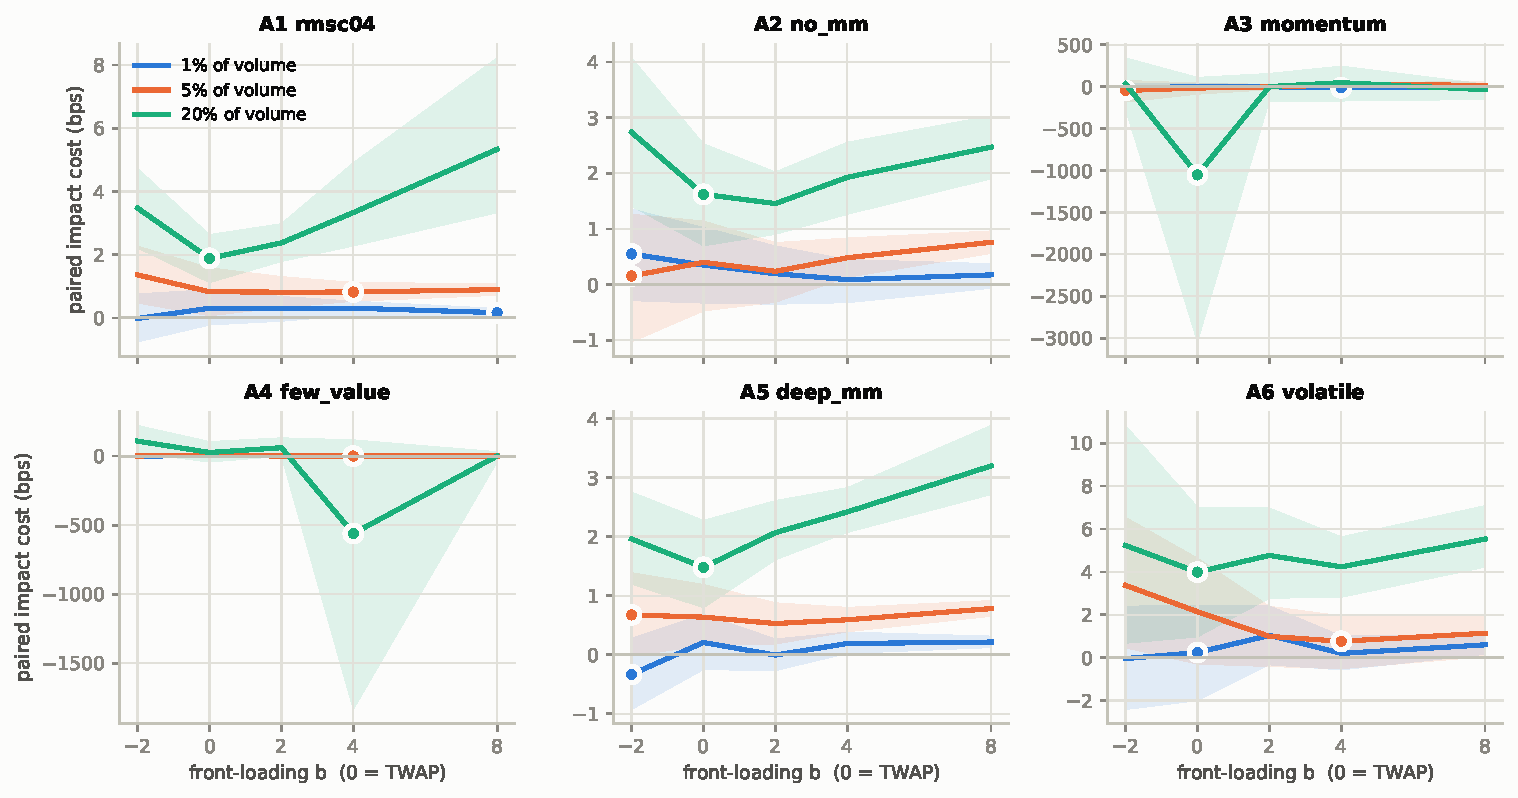
\includegraphics[width=\linewidth]{figures/fig_cost_vs_schedule.pdf}
\caption{Paired impact cost of the schedule family in each world. Bands are 95\% bootstrap intervals over \nSeeds{} seeds; the ringed marker is the schedule selected on training seeds. Vertical scales differ by two orders of magnitude between stable worlds (A1, A2, A5, A6) and unstable ones (A3, A4).}
\label{fig:cost}
\end{figure}

Table~\ref{tab:rank} summarises agreement between rankings. Across the stable worlds the mean Spearman correlation of the eight policies' costs is 0.62 at 5\% and 0.61 at 20\%, and there is not one significant reversal: no pair of policies is significantly ordered one way in one stable world and the other way in another. Including the unstable worlds lowers the correlations and produces six nominal reversals at 20\%, all involving A3 or A4.

\begin{table}[!htbp]
\centering\small
\caption{Agreement of policy rankings between worlds, over world pairs. $\rho$: Spearman correlation of the eight policies' mean costs. A policy pair is \emph{flipped} if its order differs between two worlds, and a \emph{significant reversal} if both paired 95\% intervals exclude zero with opposite signs.}\label{tab:rank}
\begin{tabular}{lrrrrr}
\toprule
Size & Mean $\rho$ & Min $\rho$ & Max $\rho$ & Mean flipped pairs & Significant reversals \\
\midrule
\multicolumn{6}{l}{\emph{All six worlds}} \\
1\% & 0.25 & -0.31 & 0.67 & 11.1 / 28 & 0 / 420 \\
5\% & 0.39 & -0.24 & 0.83 & 10.0 / 28 & 0 / 420 \\
20\% & 0.20 & -0.69 & 0.83 & 11.9 / 28 & 6 / 420 \\
\multicolumn{6}{l}{\emph{Stable worlds (A1, A2, A5, A6)}} \\
1\% & 0.25 & -0.21 & 0.62 & 11.7 / 28 & 0 / 168 \\
5\% & 0.62 & 0.19 & 0.83 & 7.2 / 28 & 0 / 168 \\
20\% & 0.61 & 0.24 & 0.83 & 7.8 / 28 & 0 / 168 \\
\bottomrule
\end{tabular}
\end{table}


\subsection{Which schedule each world recommends, and the cost of trusting the wrong world}
\label{sec:transfer}

Selecting the cheapest schedule on training seeds gives each world's recommendation $b^\star_i$; Figure~\ref{fig:regret} shows the regret $R_{ij}=C_j(b^\star_i)-C_j(b^\star_j)$ on test seeds, and Appendix~\ref{app:regret} gives the numbers.

\begin{figure}[!htbp]
\centering
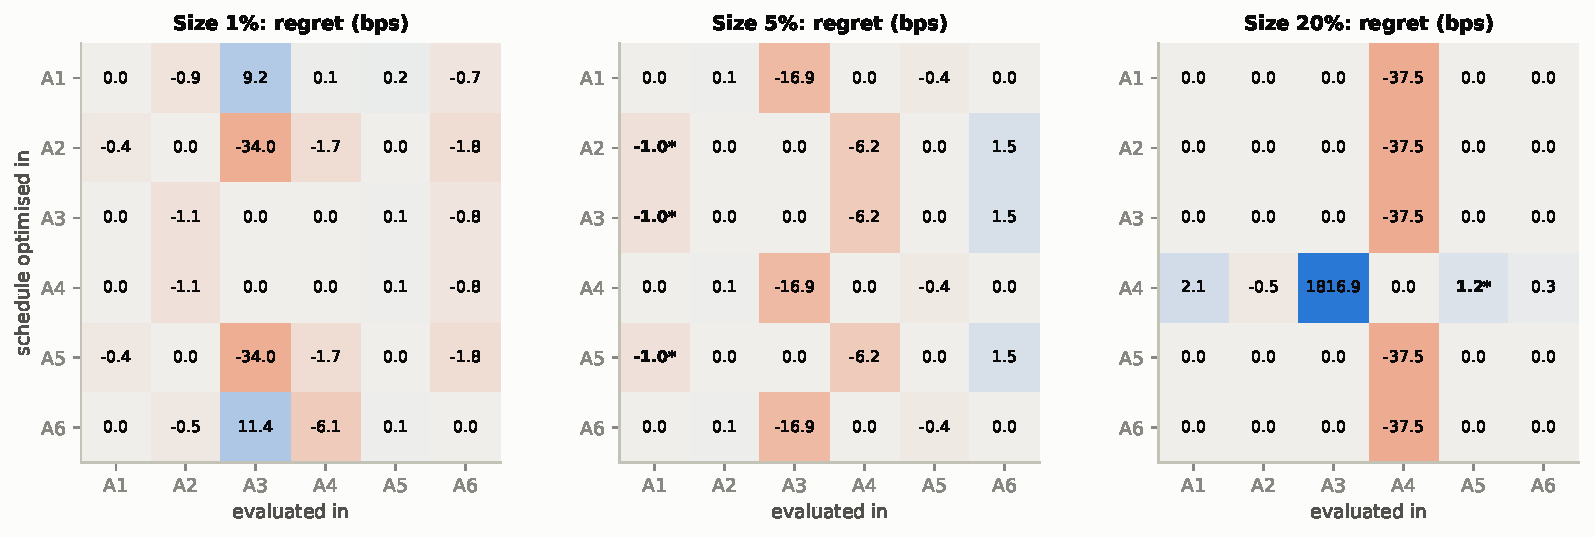
\includegraphics[width=\linewidth]{figures/fig_transfer_regret.pdf}
\caption{Transfer regret in bps (test seeds). Rows: world in which the schedule was selected. Columns: world in which it is evaluated. Bold with an asterisk: paired 95\% interval excludes zero. Colour is on a signed logarithmic scale. Negative entries arise when the schedule selected on a world's own training seeds turns out worse on its test seeds than another world's choice, i.e.\ they measure selection noise.}
\label{fig:regret}
\end{figure}

At 20\% all four stable worlds, and A3, select TWAP, so regret among them is exactly zero. At 1\% and 5\% the selected $b$ scatters across the grid (for example $-2$ in A2 and A5, $4$ in A1 and A6 at 5\%), but the scatter is selection noise on flat cost curves: among stable worlds the largest regret is \maxRegretStable{}\,bps, the mean is \meanRegretStable{}\,bps, and \nSigRegretStable{} of \nOffDiagStable{} off-diagonal regrets is significantly positive.

The only significantly positive regret in the whole matrix has an unstable world as its source: at 20\%, A4's noisy cost curve selects $b=4$, which costs 1.2\,bps more than TWAP in A5 (significant) and 2.1\,bps more in A1 (not significant). That is the practical risk in this study: not that plausible stable simulators disagree, but that an unstable one returns a confident-looking recommendation that is noise.

\subsection{Does observational distance predict transfer regret?}
\label{sec:rq4}

For each ordered pair of worlds we compare the distance between their stylised facts ($z$-scored across worlds) with the regret of transferring a schedule between them. Pooled over sizes, the Spearman correlation is \rqRhoPooled{} over \nOffDiag{} size-pair observations averaged to 30 pairs (permutation $p=\rqPPooled{}$, permuting world labels); by size it is \rqRhoOne{}, \rqRhoFive{} and \rqRhoTwenty{}. Restricted to the \rqNStable{} pairs of stable worlds it is \rqRhoStable{}. We find no evidence that observational distance predicts regret (Figure~\ref{fig:rq4}).

This is a weak test. Regret among stable worlds is at the noise floor, so there is almost nothing to predict, and six configurations of one simulator family give at most 30 dependent pairs. The result should be read as ``not detected at this resolution'', not as evidence of independence.

\begin{figure}[!htbp]
\centering
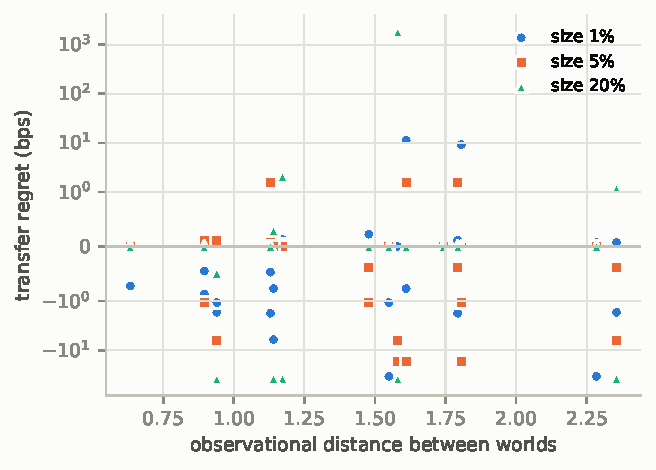
\includegraphics[width=0.6\linewidth]{figures/fig_distance_vs_regret.pdf}
\caption{Observational distance between two worlds against the regret of transferring a schedule from one to the other. The vertical axis is linear within $\pm1$\,bp and logarithmic beyond.}
\label{fig:rq4}
\end{figure}

\subsection{The MFG optimiser}
\label{sec:mfg}

Table~\ref{tab:mfg} shows the MFG calibration in each world and the schedule it prescribes through Equation~\eqref{eq:bmfg}.

\begin{table*}[!htbp]
\centering\footnotesize
\caption{MFG calibration per world (training seeds) and the schedule it prescribes, against the schedule chosen by direct search ($b^\star_{\mathrm{sim}}$, training seeds). $a$: temporary impact at the TWAP rate (bps); $\lambda$: mean mid displacement at the deadline under TWAP (bps). Costs are test-seed means in bps. $^\ast$ clipped to the grid range $[-2,8]$.}\label{tab:mfg}
\begin{tabular}{lrrrrrrr}
\toprule
World & $a$ & $\lambda$ [95\% CI] & $b_{\mathrm{MFG}}$ & $b^\star_{\mathrm{sim}}$ & $C(b_{\mathrm{MFG}})$ & $C(\mathrm{TWAP})$ & $C(b^\star)$ \\
\midrule
\multicolumn{8}{l}{\emph{Parent order = 1\% of background volume}} \\
A1 & 0.01 & 1.2 [-1.0, 3.5] & 8.0$^\ast$ & 8 & 0.1 & 0.1 & -0.3 \\
A2 & 0.02 & 0.3 [-1.7, 2.3] & 8.0$^\ast$ & -2 & 0.1 & 0.5 & -0.1 \\
A3 & -0.43 & -24.5 [-159.9, 131.4] & 8.0$^\ast$ & 4 & -8.1 & -5.9 & -51.3 \\
A4 & -0.04 & 33.0 [5.5, 69.4] & 8.0$^\ast$ & 4 & 0.3 & -6.0 & -6.0 \\
A5 & 0.00 & 0.5 [-1.7, 2.6] & 8.0$^\ast$ & -2 & 0.2 & 0.1 & -0.0 \\
A6 & 0.01 & -3.6 [-13.0, 5.1] & -2.0$^\ast$ & 0 & -0.0 & 1.8 & -0.0 \\
\multicolumn{8}{l}{\emph{Parent order = 5\% of background volume}} \\
A1 & 0.05 & 4.6 [1.9, 7.3] & 8.0$^\ast$ & 4 & 0.8 & 0.0 & -0.3 \\
A2 & 0.08 & 1.4 [-0.5, 3.5] & 8.0$^\ast$ & -2 & 0.8 & 0.0 & 0.0 \\
A3 & 0.22 & -12.3 [-117.6, 63.7] & -2.0$^\ast$ & -2 & 2.8 & -68.3 & -68.3 \\
A4 & -0.01 & 28.4 [12.1, 47.7] & 8.0$^\ast$ & 4 & -0.3 & -0.9 & -8.4 \\
A5 & 0.03 & 2.4 [0.0, 4.6] & 8.0$^\ast$ & -2 & 0.8 & 0.3 & 0.3 \\
A6 & 0.08 & 3.8 [-4.8, 11.7] & 8.0$^\ast$ & 4 & 1.5 & 2.9 & 0.5 \\
\multicolumn{8}{l}{\emph{Parent order = 20\% of background volume}} \\
A1 & 0.51 & 3.1 [1.0, 5.0] & 3.0 & 0 & 2.9 & 1.5 & 1.5 \\
A2 & 0.37 & -1.1 [-3.3, 1.2] & -1.4 & 0 & 2.4 & 2.4 & 1.6 \\
A3 & -2.13 & -1688.9 [-5207.2, 544.2] & 8.0$^\ast$ & 0 & -100.1 & -1812.1 & -1812.1 \\
A4 & -0.18 & 558.9 [14.6, 1556.5] & 8.0$^\ast$ & 4 & -22.0 & -25.2 & -25.2 \\
A5 & 0.14 & 3.0 [-0.2, 6.3] & 8.0$^\ast$ & 0 & 2.9 & 1.0 & 1.0 \\
A6 & 0.69 & 5.8 [-2.5, 15.2] & 4.2 & 0 & 4.8 & 4.4 & 0.7 \\
\bottomrule
\end{tabular}
\end{table*}


\emph{The prescription is unstable across worlds, and the instability is calibration noise.} Temporary impact at the TWAP rate is tiny (a few hundredths of a basis point at 1\% and 5\%, about half a basis point at 20\%), while the displacement $\lambda$ is a few basis points with an interval that includes zero in most stable cells. Their ratio therefore swings to the edge of the grid: $b_{\mathrm{MFG}}$ is clipped in \nMfgClipped{} of \nMfgCells{} cells. At 20\% it is 3.0 in A1, $-1.4$ in A2, 8 in A5 and 4.2 in A6, while direct search selects 0 in all four. So the answer to ``does the MFG optimiser decide differently in different worlds?'' is yes, but for a reason that has little to do with the worlds: the decision rule divides a noisy number by a small one.

\emph{Where it can be resolved, the MFG prescription is costly for a single meta-order.} In A1 and A5 at 20\%, front-loading to $b=8$ roughly doubles to triples the cost of TWAP (Table~\ref{tab:vstwap}: $+3.5$ and $+1.7$\,bps on TWAP costs of 1.9 and 1.5\,bps). This is the expected direction: the equilibrium of Section~\ref{sec:mfgmodel} describes many sellers racing each other, and a lone seller who internalises their own impact has no one to race. Injecting the equilibrium aggregate as one order prices the cost of that race. The classical single-agent, risk-neutral answer (TWAP) is what direct search recovers in every stable world at the size where the curve is resolvable.

\emph{Model structure.} Two assumptions of the linear model can be checked. Cost grows less than linearly in size in three of four stable worlds (Table~\ref{tab:impact}; exponents 0.5 to 0.7, with 0.96 in A6), in line with the concavity found empirically \citep{toth2011anomalous}; these are point estimates from three sizes. We could not estimate impact decay: five minutes after the deadline the displacement estimates are too noisy to distinguish full persistence from full reversion (Figure~\ref{fig:path}).

\begin{table*}[!htbp]
\centering\footnotesize
\caption{Shape of TWAP impact cost. Size exponent: log--log slope of mean sell cost against size over the three sizes (1 = linear, 0.5 = square-root); a point estimate from three sizes, not reported for unstable worlds. Buy$-$sell: paired difference in cost (bps) with 95\% interval.}\label{tab:impact}
\begin{tabular}{lrrrr}
\toprule
World & Size exponent (sell) & Buy$-$sell, 1\% & Buy$-$sell, 5\% & Buy$-$sell, 20\% \\
\midrule
A1 & 0.61 & -0.8 [-1.6, 0.0] & -0.9 [-2.1, 0.3] & 0.0 [-1.2, 1.2] \\
A2 & 0.50 & 0.3 [-1.0, 1.5] & -0.7 [-2.0, 0.8] & -0.4 [-1.9, 1.0] \\
A3 & -- & 309.8 [-73.4, 1016.6] & 15.6 [-78.7, 114.0] & 1564.9 [214.2, 3671.7] \\
A4 & -- & -9.6 [-28.5, 5.4] & -4.2 [-10.6, 3.1] & 166.6 [-26.6, 477.5] \\
A5 & 0.66 & 0.0 [-0.7, 0.8] & 0.2 [-0.6, 1.0] & 1.1 [-0.1, 2.1] \\
A6 & 0.96 & -1.2 [-4.3, 1.8] & -2.0 [-6.3, 2.0] & -1.0 [-5.5, 3.5] \\
\bottomrule
\end{tabular}
\end{table*}


\begin{figure}[!htbp]
\centering
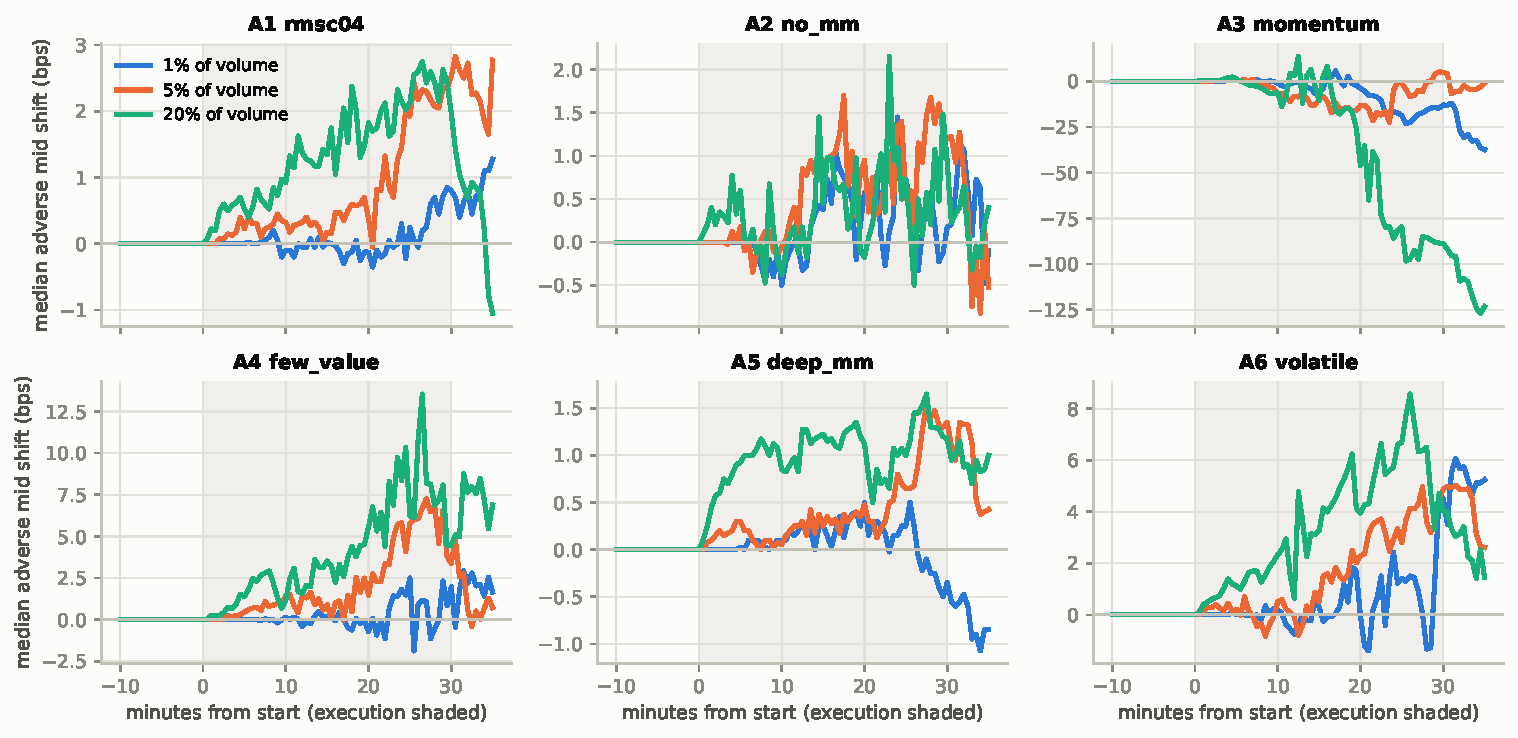
\includegraphics[width=\linewidth]{figures/fig_impact_path.pdf}
\caption{Median adverse displacement of the mid price relative to the twin, during and after a TWAP sell. A positive value means the price is lower than it would have been.}
\label{fig:path}
\end{figure}

\emph{Buy versus sell.} No stable world shows a significant difference between the cost of buying and selling at any size (Table~\ref{tab:impact}).

\subsection{TRADES arm}
\label{sec:tradesresults}

The TRADES arm is small: \tradesSeeds{} seeds, each with an unperturbed twin and five interventions (\nTradesEpisodes{} episodes of about \tradesWall{} minutes each). The parent order is \tradesQty{} shares, 10\% of the generated market's mean volume in the 10-minute window. Twin and intervention were identical before the first child order in \tradesPreIdentical{} of runs and differed afterwards in all of them, so the generated flow does respond to the injected orders.

\begin{table*}[!htbp]
\centering\footnotesize
\caption{The 10-minute task (sell 10\% of background volume in 20 slices) in every ABIDES world and in the retrained TRADES market T1. Paired impact cost in bps, mean $\pm$ 95\% half-width. Bold: cheapest schedule in each column.}\label{tab:short}
\begin{tabular}{lrrrrrrr}
\toprule
Policy & A1 & A2 & A3 & A4 & A5 & A6 & T1 \\
\midrule
Schedule $b=-2$ (back-loaded) & 0.7{\tiny$\,\pm$0.2} & \textbf{0.4{\tiny$\,\pm$0.3}} & 11.8{\tiny$\,\pm$9.1} & 1.0{\tiny$\,\pm$1.1} & \textbf{0.5{\tiny$\,\pm$0.2}} & 1.2{\tiny$\,\pm$1.2} & 41.6{\tiny$\,\pm$21.2} \\
Schedule $b=0$ (TWAP) & 0.7{\tiny$\,\pm$0.3} & 0.4{\tiny$\,\pm$0.3} & 4.6{\tiny$\,\pm$10.8} & 1.2{\tiny$\,\pm$1.2} & 0.6{\tiny$\,\pm$0.2} & 0.8{\tiny$\,\pm$0.7} & 50.6{\tiny$\,\pm$27.2} \\
Schedule $b=2$ & \textbf{0.5{\tiny$\,\pm$0.3}} & 0.6{\tiny$\,\pm$0.3} & 4.4{\tiny$\,\pm$6.3} & \textbf{0.7{\tiny$\,\pm$0.6}} & 0.6{\tiny$\,\pm$0.1} & \textbf{0.3{\tiny$\,\pm$0.6}} & 44.2{\tiny$\,\pm$28.8} \\
Schedule $b=8$ (front-loaded) & 1.1{\tiny$\,\pm$0.3} & 1.2{\tiny$\,\pm$0.3} & \textbf{3.8{\tiny$\,\pm$2.3}} & 1.5{\tiny$\,\pm$0.6} & 0.7{\tiny$\,\pm$0.1} & 1.6{\tiny$\,\pm$0.6} & \textbf{26.6{\tiny$\,\pm$16.6}} \\
Immediate & 2.1{\tiny$\,\pm$0.4} & 1.9{\tiny$\,\pm$0.5} & 5.3{\tiny$\,\pm$2.3} & 2.5{\tiny$\,\pm$0.9} & 1.1{\tiny$\,\pm$0.2} & 4.5{\tiny$\,\pm$1.4} & 15.7{\tiny$\,\pm$2.4} \\
\midrule
Episodes per cell & 40 & 40 & 40 & 40 & 40 & 40 & 6 \\
\bottomrule
\end{tabular}
\end{table*}


Table~\ref{tab:short} puts the TRADES market next to the ABIDES worlds on the identical task. The two families give opposite advice. In every stable ABIDES world the immediate order is clearly the most expensive policy and the schedules are close to one another. In the TRADES market the ordering is reversed: the immediate order and the most front-loaded schedule are the cheapest, at \tradesCostImm{}\,bps and \tradesCostFront{}\,bps ($b=8$), and TWAP is the most expensive, at \tradesCostTwap{}\,bps. Paired by seed, $b=8$ differs from TWAP by \tradesDiffFront{}\,bps (95\% interval \tradesDiffFrontCI{}; cheaper in \tradesDiffFrontN{} seeds), and the immediate order by \tradesDiffImm{}\,bps (\tradesDiffImmCI{}). The estimates are noisy: two seeds have TWAP costs near 100\,bps. The generated market is also far more impact-sensitive than any ABIDES world: selling 10\% of volume shifts the mid by \tradesDispMin{} to \tradesDispMax{}\,bps by the deadline depending on the schedule, against at most \abidesShortDispMax{}\,bps under TWAP in the stable ABIDES worlds, and the shift under TWAP is still \tradesDispTwapPost{}\,bps two minutes later. Selecting the schedule in the TRADES market and deploying it in a stable ABIDES world costs between \tradesToAbidesMin{} and \tradesToAbidesMax{}\,bps of regret; selecting in a stable ABIDES world and deploying in the TRADES market costs between \abidesToTradesMin{} and \abidesToTradesMax{}\,bps. These are point estimates from \tradesSeeds{} seeds with no train/test split.

So here is a pair of simulators that do disagree materially. The disagreement, however, has a mundane source, and it is one that realism statistics catch. The retrained generator does not hold the market it inherits. Across unperturbed twins the quoted spread is \tradesSpreadReplay{}\,bps in the last minute of real replay, \tradesSpreadFirst{}\,bps in the first generated minute, \tradesSpreadMid{}\,bps after five minutes and \tradesSpreadLast{}\,bps in the last minute of the task. A seller who trades early crosses a spread close to the real one; a seller who waits crosses a spread several times wider. Front-loading wins because the simulated market deteriorates with time since hand-over, not because of anything about impact. Table~\ref{tab:tradesreal} shows the same thing in aggregate: over the task window the generated market's spread and volatility are well above those of the real day it was trained on.

\begin{table}[!htbp]
\centering\small
\caption{Unperturbed retrained-TRADES market against the real day it was trained on, over the task window. The real window lies in the training split.}\label{tab:tradesreal}
\begin{tabular}{lrrr}
\toprule
Statistic (09:46--09:56) & TRADES mean & TRADES s.d. & Real INTC \\
\midrule
Quoted spread (bps) & 24.06 & 13.23 & 3.66 \\
10\,s return volatility (bps) & 7.29 & 1.25 & 3.92 \\
Return autocorrelation, lag 1 & -0.38 & 0.09 & -0.15 \\
$|$return$|$ autocorrelation, lag 1 & 0.23 & 0.08 & -0.15 \\
Traded volume (shares) & 315618 & 39337 & 247627 \\
\bottomrule
\end{tabular}
\end{table}


We stress what this does and does not show. It is evidence about a TRADES architecture trained for \tradesSteps{} steps on one day, and says nothing about the published model. But it illustrates the second way, besides instability, in which a simulator can mislead an execution study: a generator whose state drifts away from its conditioning imposes a time preference of its own on every schedule evaluated inside it. A spread-versus-time plot of unperturbed runs is enough to detect it.


\section{Discussion}

\paragraph{What the evidence supports.} Among the four stable ABIDES configurations we could not detect disagreement about which execution schedule is best. Rankings correlate at about 0.6 once the order is large enough to measure, there are no significant reversals, all four select TWAP at 20\% of volume, and the largest transfer regret is \maxRegretStable{}\,bps. The configurations do differ in how steeply they penalise urgency, by a factor of about four between the reference world and the world without market makers, so they would disagree about a risk-averse trader's trade-off even though they agree about a risk-neutral one. We did not run that experiment.

\paragraph{Where simulators did disagree.} The one material disagreement in the study is between families: the retrained TRADES market favours selling at once, every stable ABIDES world favours spreading, and carrying an ABIDES-selected schedule into the TRADES market costs \abidesToTradesMin{} to \abidesToTradesMax{}\,bps on point estimates. We do not read this as a property of diffusion-based generators. The TRADES arm differs from the ABIDES arm in stock, price level, calibration and training budget at once, and the direct cause, a spread that widens with time since hand-over, is a defect of an under-trained model. What transfers is the diagnostic: a simulator can impose a time preference of its own, and it shows up in unperturbed runs.

\paragraph{What it does not support.} The hypothesis that motivated the study, that plausible simulators recommend materially different schedules, is not supported for these configurations at this resolution. We also cannot claim they are equivalent: the intervals in Table~\ref{tab:cost} would hide differences of one or two basis points at 5\% and several at 20\% in A6. And six configurations of one simulator, sharing an exchange and most of their agents, are a narrow sample of ``plausible simulators''.

\paragraph{Stability before realism.} The most useful practical finding is the cheapest one to check. Two configurations obtained by changing a single population parameter of the reference configuration produce markets whose unperturbed price paths are too wild for any execution experiment, and one of them contains seeds that never terminate. Neither is flagged by spread, kurtosis or volatility clustering, and both sit nearer to the real reference day than the stable worlds do. An unperturbed-stability check, and a twin-pairing noise check like Table~\ref{tab:noise}, cost a few hundred episodes and should precede any policy evaluation.

\paragraph{On the MFG as a decision rule.} Calibrating a two-parameter impact model from probe trades and reading the schedule off a closed form is attractive because it is cheap. In these simulators it is also fragile: the schedule depends on a ratio whose numerator is statistically indistinguishable from zero in most cells. Direct search over the same schedule family, with paired twins, used the same episodes and gave a stable answer.

\section{Limitations}
\label{sec:limits}

\begin{itemize}[leftmargin=*,itemsep=2pt]
\item \textbf{No real-market ground truth.} Regret is simulator-to-simulator. We cannot say which world is right, only whether they agree. The single INTC day is a reference point for stylised facts, not a validation.
\item \textbf{One simulator family.} All ABIDES worlds share an exchange, an oracle and most agent code; TRADES runs inside a legacy ABIDES exchange. ABIDES-MARL is absent because we found no public code.
\item \textbf{TRADES is our retraining, not the published model.} It was trained for \tradesSteps{} steps on one stock-day; its conclusions do not transfer to the authors' checkpoints. The TRADES and ABIDES arms differ in stock, price level, tick-to-price ratio and calibration, so differences between them cannot be attributed to the generator.
\item \textbf{Statistical power.} \nSeeds{} seeds, split in half for selection and evaluation. Differences below roughly 1\,bp at 5\% and 1 to 3\,bps at 20\% are not detectable in stable worlds, and nothing is detectable in unstable ones. No multiplicity correction was applied.
\item \textbf{Narrow policy class.} Market orders only, a five-point schedule grid, no limit orders, no fees, no reinforcement learning, risk-neutral objective.
\item \textbf{Post-hoc choices.} The stability rule was set after seeing the data, and two configurations were changed during piloting for runtime reasons (36 instead of 60 momentum traders; market makers at the default instead of a 10-second refresh interval). Runaway seeds are excluded, which conditions on an outcome.
\item \textbf{MFG simplification.} We test the risk-neutral homogeneous equilibrium injected as one meta-order. Heterogeneous beliefs, latent alpha and filtering, which are the substance of \citet{casgrain2020mean}, are not exercised.
\item \textbf{Novelty.} We ran targeted searches, not a systematic review, and make no claim to be first.
\end{itemize}

\section{Conclusion}

We set out to show that plausible market simulators recommend different trades. For four stable ABIDES configurations they do not, as far as \nSeeds{} paired seeds can tell: they agree that an order of 20\% of volume should be spread evenly, and that below that size the schedule barely matters as long as the order is not sent all at once. Two further configurations, one parameter away from the reference, are too unstable to say anything, and conventional realism statistics do not reveal it. An MFG calibrated per world does give different answers in different worlds, but the differences are calibration noise, and its front-loaded prescription is measurably worse than TWAP for a single order. A TRADES market retrained on one day of data recommends the opposite of ABIDES, for a reason that has to do with the generator drifting and not with execution. The harness, the paired-twin estimator and all results are released so the comparison can be extended to simulators we could not run.
